\subsection{功能三 司机任务执行与模拟位置共享}
\owner{赵凯彭}
司机端围绕一次行程组织任务列表、乘客名单、上车点和位置共享状态。其主要难点是协调任务生命周期与定时器生命周期：发车后生成位置记录，到站后停止生成，并保证同一时刻只有一个活动任务。

\subsubsection{场景建模}
\begin{table}[H]\centering\small
\caption{司机执行任务与位置共享用例描述}
\begin{tabularx}{\linewidth}{|P{2cm}|Y|}\hline
用例名称 & UC-D01 执行派车任务并共享模拟位置\\\hline
参与者 & 已登录司机工作台的司机\\\hline
前置条件 & 已加载演示任务；目标任务尚未完成；当前没有活动任务。\\\hline
触发事件 & 司机核对任务后点击开始任务。\\\hline
基本流程 & （1）查看车次、路线、发车时间和乘客数；（2）展开乘客名单及上车点；（3）开始任务；（4）任务状态改为行程中并记录活动任务标识；（5）立即生成首条位置，此后每5秒生成一条；（6）到站后完成任务；（7）任务改为已完成，停止定时器并清除活动任务。\\\hline
异常流程 & 已有活动任务、任务不存在或任务已完成时拒绝开始；没有活动任务时不能完成任务。\\\hline
后置条件 & 任务状态与位置共享状态一致；已完成任务不能再次发车；已有位置记录保留供页面查看。\\\hline
关联操作 & 切换日、周、月统计维度，查看对应预置统计数据。\\\hline
\end{tabularx}\end{table}
界面中的位置上报通过本地坐标序列模拟。5秒代表定时生成记录的间隔，能够用于检查状态更新和交互流程；真实 GPS 权限、后台定位、网络上传和管理员订阅需要在后续联调中完成。

\subsubsection{类建模}
图\ref{fig:driver-class}以任务状态为中心组织乘客上车信息与位置记录。任务内包含乘客列表，位置记录通过车辆标识对应车辆；控制器保存活动任务标识和位置列表。
\begin{figure}[H]\centering
\begin{tikzpicture}[x=1cm,y=1cm]
\node[box,text width=5.9cm] (task) at (0,0) {\textbf{DriverTaskModel}\par\rule{5.7cm}{0.3pt}\par\code{id, tripNo, vehicleId, driverId}\par\code{routeName, departureTime}\par\code{passengers, status}};
\node[box,text width=5.9cm] (pickup) at (7.3,0) {\textbf{PassengerPickup}\par\rule{5.7cm}{0.3pt}\par\code{name, phoneSuffix}\par\code{pickupPoint, seatNo}};
\node[box,text width=5.9cm] (state) at (0,-4.0) {\textbf{DriverTaskState}\par\rule{5.7cm}{0.3pt}\par\code{tasks, activeTaskId?}\par\code{locationUpdates, stats}\par\code{latestLocation, activeTask}};
\node[box,text width=5.9cm] (loc) at (7.3,-4.0) {\textbf{LocationUpdate}\par\rule{5.7cm}{0.3pt}\par\code{vehicleId, lat, lng}\par\code{speed, timestamp}};
\draw (task.east)--node[font=\scriptsize,above]{1\quad 0..*}(pickup.west);
\draw (state.north)--node[font=\scriptsize,left,pos=.2]{1}node[font=\scriptsize,left,pos=.8]{0..*}(task.south);
\draw (state.east)--node[font=\scriptsize,above]{1\quad 0..*}(loc.west);
\end{tikzpicture}
\caption{司机任务与位置记录类模型（字段节选）}\label{fig:driver-class}
\end{figure}

\noindent\textbf{模型分工。}\code{DriverTaskModel}描述任务及当前状态；\code{PassengerPickup}保存姓名、手机号尾号、上车点和座位号；\code{LocationUpdate}保存车辆标识、经纬度、速度与时间；\code{DriverStats}保存日、周、月预置统计。\code{DriverTaskState}集中保存上述数据和\code{activeTaskId}，页面据此决定可执行操作。

\subsubsection{功能建模/行为建模}
图\ref{fig:driver-state}展示任务状态和共享动作之间的对应关系。任务开始后立即产生首条位置，再周期更新；完成时关闭定时器，并在 Provider 销毁时执行同样的清理动作。
\begin{figure}[H]\centering
\begin{tikzpicture}[x=1cm,y=1cm,font=\small]
\node[circle,fill=black,minimum size=5pt,inner sep=0] (s) at (-1,0) {};
\node[state,text width=2.6cm] (p) at (1.5,0) {待发车\par pending};
\node[state,text width=2.6cm] (r) at (6.5,0) {行程中\par running};
\node[state,text width=2.6cm] (c) at (11.5,0) {已完成\par completed};
\draw[flow] (s)--(p);
\draw[flow] (p)--node[smalllabel,above,align=center]{开始任务\\无活动任务}(r);
\draw[flow] (r)--node[smalllabel,above]{到站完成}(c);
\node[box,text width=4.8cm,align=center] (timer) at (6.5,-2.4) {进入时：立即生成位置\par 运行时：每5秒追加记录\par 离开时：取消定时器};
\draw[dashed] (r)--(timer);
\node[box,text width=3.0cm,align=center] at (0.7,-2.4) {已有活动任务：拒绝开始\par 任务不存在：返回错误};
\node[box,text width=2.5cm,align=center] at (11.8,-2.4) {已完成任务\par 不可再次发车};
\end{tikzpicture}
\caption{司机任务状态及位置定时器生命周期}\label{fig:driver-state}
\end{figure}

\noindent\textbf{关键不变条件。}
\begin{enumerate}
\item \code{activeTaskId}最多指向一个任务。已有活动任务时拒绝再次开始，避免并行创建多个位置定时器。
\item 位置信息由当前活动任务决定车辆标识。没有活动任务时，手动模拟位置操作直接返回。
\item 完成任务后，任务状态改为\code{completed}，定时器取消，活动任务标识清空；保留已生成记录，便于核对运行结果。
\item 控制器通过\code{ref.onDispose(_stopTimer)}清理资源，避免 Provider 生命周期结束后继续触发更新。
\end{enumerate}
当前位置由基础坐标与记录步数计算：纬度每步增加0.0018，经度每步增加0.0012，速度按步数周期变化。该规则使界面可以稳定演示“位置变化—最近更新时间—记录列表”的效果，不据此计算真实里程、定位精度或网络时延。

\subsubsection{代码结构及说明}
\begin{table}[H]\centering\small
\caption{司机任务与位置共享代码结构}
\begin{tabularx}{\linewidth}{|P{2.1cm}|Y|}\hline
层次 & 文件与职责\\\hline
页面层 & \code{lib/features/driver/presentation/driver_home_page.dart}：任务卡片、乘客展开列表、统计面板和位置共享面板。\\\hline
状态层 & \code{lib/features/driver/tasks/providers/driver_task_provider.dart}：开始/完成任务、生成位置记录、统计切换和定时器管理。\\\hline
数据层 & \code{lib/features/driver/tasks/data/mock_driver_repository.dart}：提供初始任务、乘客和统计数据。\\\hline
模型层 & \code{lib/core/models/driver_task_model.dart}与\code{location_update.dart}：任务、上车信息、统计和位置结构。\\\hline
\end{tabularx}\end{table}

\noindent\textbf{关键实现。}\code{startTask}先检查活动任务和目标任务，再更新状态并创建定时器；\code{completeActiveTask}负责完成与停止。下面摘录定时更新与资源清理部分：
\begin{source}
// In build(): clean up when the provider is disposed.
ref.onDispose(_stopTimer);

// In startTask(): after updating task and activeTaskId.
_appendLocationUpdate();
_locationTimer = Timer.periodic(const Duration(seconds: 5), (_) {
  _appendLocationUpdate();
});

void _stopTimer() {
  _locationTimer?.cancel();
  _locationTimer = null;
}
\end{source}
\noindent\textbf{阶段验证。}\code{test/driver_test.dart}覆盖任务卡片、统计切换、乘客展开、开始任务、模拟上报和到站完成等内容。验证重点是开始后产生首条记录、重复开始被拦截、完成后不继续增加位置、已完成任务不可重启。下一阶段应继续检查页面切换、退出登录和异常中断时的资源清理，以及真实定位数据的过期判断。

\clearpage
\subsubsection{界面截图}
\begin{figure}[H]\centering
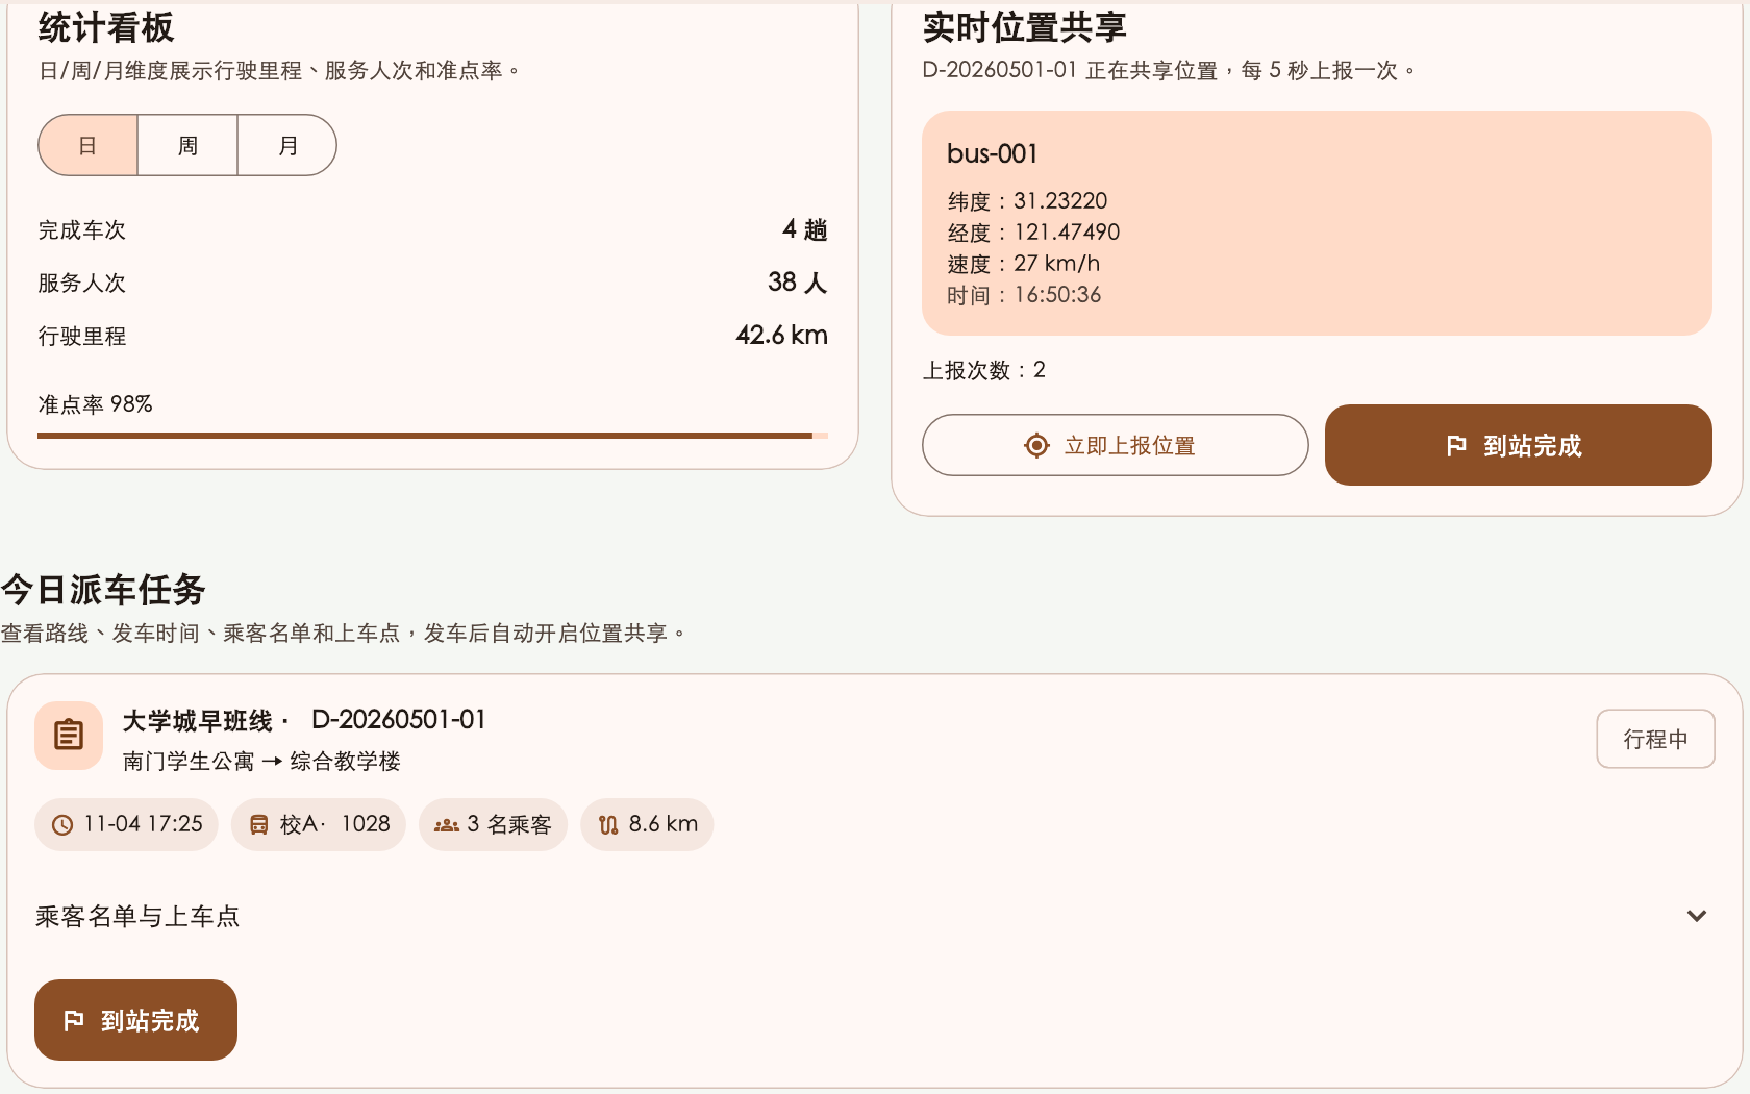
\includegraphics[width=\linewidth,height=0.64\textheight,keepaspectratio]{figures/driver.pdf}
\caption{司机任务行程中与模拟位置上报的运行界面}\label{fig:driver-screen}
\end{figure}

司机工作台将任务执行状态与位置共享状态放在同一页面。任务卡片提供路线、发车时间和乘客信息，司机开始任务后可看到当前车辆、坐标、速度和最近上报时间；到站完成后共享停止，任务状态相应改变。

本阶段已建立任务状态与模拟位置记录联动的基础，并完成日、周、月统计展示。后续将以共享服务端为连接点，统一后台确认方案与司机任务的数据来源，再逐步接入真实定位与通信；同时完善乘客预约、后台调度和司机执行之间的数据一致性验证。
